\chapter{Introducci\'{o}n y antecedentes}
\epigraph{You do not really understand something unless you can explain it to your grandmother.}{Albert Einstein}

En este cap\'{i}tulo se brinda una breve descripci\'{o}n de por qu\'{e} es necesaria la creaci\'{o}n de t\'{e}cnicas baratas y r\'{a}pidas de reconstrucci\'{o}n tridimensional. Posteriormente, se introducen conceptos b\'{a}sicos relacionados con la visi\'{o}n artificial, el problema de la reconstrucci\'{o}n y por qu\'{e} es tan dif\'{i}cil de resolver. Luego, se detallan las tres grandes \'{a}reas en las que generalmente se divide todo proceso de reconstrucci\'{o}n tridimensional. Finalmente, se detalla una secci\'{o}n de trabajo relacionado.


\section{Motivaci\'{o}n}
La demanda por modelos tridimensionales (3D) virtuales de objetos f\'{i}sicos complejos ha venido en crecimiento en una gran cantidad de \'{a}reas. Modelos 3D de gran realismo son utilizados a diario para visualizar y simular eventos en el campo m\'{e}dico \cite{McInerney_Terzopoulos_1996,Chen_Hou_Gou_Lu_2000}, en simuladores de vuelo \cite{Baarspul_1990}, en juegos \cite{Freeman_Tanaka_Ohta_Kyuma_1996}, arquitectura \cite{Werner_Zisserman_2002}, en la industria f\'{i}lmica \cite{wiki:Walle}, impresi\'{o}n 3D \cite{japanese1996jtec}, entre otros. Una de las grandes limitantes para el uso generalizado de este tipo de t\'{e}cnicas es el costo elevado de estos modelos 3D dado que son producidos manualmente. Si los objetos a reconstruir provienen del mundo real, el proceso implica planificar un conjunto de vistas, alterar y manipular f\'{i}sicamente la posici\'{o}n del objeto y del sensor, realizar capturas del objeto, registrar los datos geom\'{e}tricos adquiridos en un marco de referencia com\'{u}n, y finalmente, integrar la informaci\'{o}n adquirida en un modelo virtual consistente y no redundante \cite{Jahne_Haussecker_Geibler_1999,Faugeras_1993,Faugeras_Luong_2001,Szeliski_2010}. Dada la naturaleza de este proceso, validar la correctitud del modelo generado implica mucho tiempo, esfuerzo y dinero.

En la actualidad, la visi\'{o}n artificial provee t\'{e}cnicas activas o pasivas para obtener medidas tridimensionales de una escena u objeto a reconstruir \cite{Herbort_Wohler_2011,Szeliski_2010,Forsyth_Ponce_2002,Cyganek_Siebert_2009}. Con t\'{e}cnicas activas, un tipo de energ\'{i}a como la luz l\'{a}ser o in\-fra\-rro\-ja, es proyectada sobre el objeto y la energ\'{i}a reflejada es utilizada para calcular las mediciones 3D \cite{Rocchini_Cignoni_Montani_Pingi_Scopigno_2001,Cui_Schuon_Chan_Thrun_Theobalt_2010,Smisek_Jancosek_Pajdla_2011}. Usualmente, este tipo de sensores brindan medidas de mayor precisi\'{o}n a expensas de equipo costoso especializado y de un rango de profundidad limitado en la captura. Por otro lado, las t\'{e}cnicas pasivas se basan \'{u}nicamente en el contenido natural brindado por una c\'{a}mara \cite{Szeliski_2010,Faugeras_Luong_2001,Pollefeys_Gool_2002,Faugeras_1992}. Debido a esto, no pueden garantizar medidas tan precisas como las de t\'{e}cnicas activas. La gran ventaja de las t\'{e}cnicas pasivas es el bajo costo de adquisici\'{o}n del equipo (una o dos c\'{a}maras es suficiente) y el amplio rango de profundidad en la captura, limitado solo por el desplazamiento de las c\'{a}maras.

Esta tesis muestra una t\'{e}cnica r\'{a}pida de reconstrucci\'{o}n tridimensional, la cual convierte r\'{a}pidamente pares de im\'{a}genes estereosc\'{o}picas bidimensionales de un objeto del mundo real en una representaci\'{o}n tridimensional de \'{e}ste, conocida como nube densa de puntos 3D. Las im\'{a}genes son capturadas utilizando una c\'{a}mara de bajo costo tipo \textit{webcam} y una base giratoria de madera. Con dicha t\'{e}cnica se pretende reducir la duraci\'{o}n as\'{i} como los costos del proceso de reconstrucci\'{o}n, al no requerir de equipo ni personal especializado.

Tradicionalmente, en reconstrucci\'{o}n tridimensional se utiliza el pareo de caracter\'{i}sticas sobresalientes (del ingl\'{e}s \textit{feature matching}) en lugar de t\'{e}cnicas de rastreo denso debido a que se considera m\'{a}s r\'{a}pido y funciona mejor para im\'{a}genes con una separaci\'{o}n espacial grande \cite{Liu_Cheng_2008,Peng_Chen_Zhou_Liu_2009,Wang_Quan_2008,Ying_Hong-e_Ben-zhi_2010}. El problema de esta t\'{e}cnica es que el resultado de la reconstrucci\'{o}n es dispersa (pocos puntos tridimensionales) y no se desempe\~na bien cuando la separaci\'{o}n espacial entre im\'{a}genes es peque\~na.

La novedad de la t\'{e}cnica propuesta es que utiliza algoritmos de rastreo denso de pixeles en conjunto con una t\'{e}cnica pir\'{a}mide para el r\'{a}pido procesamiento de las im\'{a}genes y una r\'{a}pida triangulaci\'{o}n para la generaci\'{o}n de la informaci\'{o}n tridimensional. Generalmente, el rastreo denso no es apto para ser utilizado en reconstrucci\'{o}n r\'{a}pida debido a la cantidad considerable de datos que hay que procesar, sin embargo la t\'{e}cnica propuesta se basa en un algoritmo lineal reciente que permite obtener resultados de gran calidad en cuesti\'{o}n de unos cuantos segundos y sin la utilizaci\'{o}n de equipo especializado.


\section{Visi\'{o}n artificial}
De acuerdo con \cite{university1995binocular}, las primeras personas conocidas que investigaron el fen\'{o}meno de la percepci\'{o}n de la profundidad fueron los \textit{Antiguos Griegos}. Probablemente el primer escrito relacionado con el tema de disparidad proviene de Arist\'{o}teles (380 AC), quien observ\'{o} que si se presiona con un dedo uno de los globos oculares despu\'{e}s de realizar una observaci\'{o}n prolongada de un objeto, el objeto se experimenta en visi\'{o}n doble \cite{Cyganek_Siebert_2009}. Desde entonces una gran cantidad de investigadores del campo de la matem\'{a}tica, la geometr\'{i}a y la visi\'{o}n humana han influenciado y dado forma a lo que hoy conocemos como visi\'{o}n artificial.

La visi\'{o}n artificial o visi\'{o}n por computador (del ingl\'{e}s \textit{computer vision}) es un subcampo de la inteligencia artificial. Su prop\'{o}sito es describir la informaci\'{o}n contenida en una o varias im\'{a}genes y as\'{i} reconstruir propiedades tales como forma, tamaño, distancia, iluminaci\'{o}n y distribuci\'{o}n del co\-lor \cite{Szeliski_2010,Shah_1983,Shapiro_Stockman_2001,Cyganek_Siebert_2009}. La visi\'{o}n artificial incluye m\'{e}todos para adquirir, procesar, analizar y entender el contenido de im\'{a}genes digitales, con tal de producir informaci\'{o}n num\'{e}rica o simb\'{o}lica, por ejemplo en forma de decisiones \cite{Shapiro_Stockman_2001,Jahne_Haubecker_Ray_2002}. Un tema en desarrollo de este campo es replicar las habilidades de la visi\'{o}n humana al percibir y entender digitalmente una imagen \cite{Sonka_Hlavac_Boyle_2007}.

Los objetivos t\'{i}picos de la visi\'{o}n artificial incluyen:
\begin{itemize*}
\item La detecci\'{o}n, segmentaci\'{o}n, localizaci\'{o}n y reconocimiento de ciertos objetos en im\'{a}genes (por ejemplo, caras humanas). 
\item La evaluaci\'{o}n de los resultados (por ejemplo, segmentaci\'{o}n, registro). 
\item Registro de diferentes im\'{a}genes de una misma escena u objeto, es decir, hacer concordar un mismo objeto en diversas im\'{a}genes. 
\item Seguimiento de un objeto en una secuencia de im\'{a}genes. 
\item Mapeo de una escena para generar un modelo tridimensional. Este modelo podr\'{i}a ser usado por un robot para navegar por la escena. 
\item Estimaci\'{o}n de las posturas tridimensionales de humanos. 
\item B\'{u}squeda de im\'{a}genes digitales por su contenido. 
\end{itemize*}

Para cumplir estos objetivos se utiliza el reconocimiento de patrones, aprendizaje estad\'{i}stico, geometr\'{i}a de proyecci\'{o}n, procesado de im\'{a}genes, teor\'{i}a de grafos y otros campos \cite{Cryer_Shah_1999,Faugeras_1993,Cyganek_Siebert_2009,Forsyth_Ponce_2002,Hartley_Zisserman_2003}.



%\begin{figure}[htp]
%\centering
%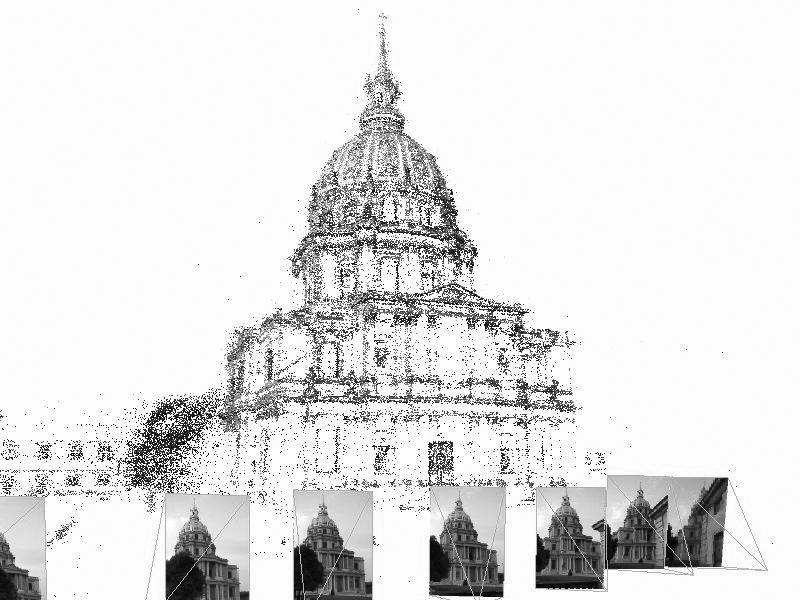
\includegraphics[scale=0.43]{images/eglise.jpg}
%\caption[Reconstrucci\'{o}n tridimensional de la \emph{Iglesia del Domo} en Paris]%
%{Con la t\'{e}cnica de \emph{estructura a partir del movimiento} es posible reconstruir estructuras como la \emph{Iglesia del Domo} en Paris utilizando \'{u}nicamente una secuencia de im\'{a}genes. Imagen de Carl Olsson \copyright \cite{olsson-etal-2011}.}
%\label{fig:Eglise}
%\end{figure}

%Una gran variedad de t\'{e}cnicas y algoritmos han sido creados para lidiar particularmente con problemas del campo de la visi\'{o}n artificial \cite{Cryer_Shah_1999,Faugeras_1993,Cyganek_Siebert_2009,Forsyth_Ponce_2002}. Por ejemplo, la detecci\'{o}n de caracter\'{i}sticas sobresalientes (del ingl\'{e}s \textit{feature detection}) permite encontrar informaci\'{o}n en im\'{a}genes la cual puede ser identificada posteriormente en otras im\'{a}genes de la misma escena. Al combinar este tipo de técnicas con

%Dos de las técnicas más desafiantes en el campo de la visión artificial son la

%La detección del flujo (del ingl\'{e}s \textit{optical flow})
%, \textit{visi\'{o}n estereosc\'{o}pica} (del ingl\'{e}s \textit{stereo vision}), \textit{estructura a partir del movimiento} (del ingl\'{e}s \textit{structure from motion}), permiten estimar la posici\'{o}n de puntos tridimensionales a partir de una secuencia de im\'{a}genes, los cuales pueden ser utilizados a su vez para determinar la geometr\'{i}a tridimensional del objeto o escena \cite{Faugeras_Luong_2001,Bay_Ess_Tuytelaars_Vangool_2008,Brostow_Shotton_Fauqueur_Cipolla_2008,Hartley_Zisserman_2003,Labatut_Pons_Keriven_2007,Cryer_Shah_1999}. Por ejemplo, la figura ~\ref{fig:Eglise} muestra una fase del proceso de reconstrucci\'{o}n tridimensional de la \emph{Iglesia del Domo} en Paris utilizando la t\'{e}cnica de \emph{estructura a partir del movimiento}, 85 c\'{a}maras y un total de 84792 puntos de la escena \cite{olsson-etal-2011}.


\subsection{¿Por qu\'{e} la visi\'{o}n artificial es tan dif\'{i}cil?}
En la visi\'{o}n artificial, una computadora recibe una matriz de n\'{u}meros que re\-pre\-senta la imagen capturada por la c\'{a}mara y nada m\'{a}s \cite{Shah_1983,Bradski_Kaehler_2008,Szeliski_2010,Cyganek_Siebert_2009}. No existen mecanismos empotrados que permitan reconocer patrones, no existen mecanismos automatizados que permitan controlar la apertura o el enfoque del lente, y finalmente, no existe un control cruzado de asociaciones hacia años de experiencia como en el caso de un ser humano.

\begin{figure}[H]
\centering
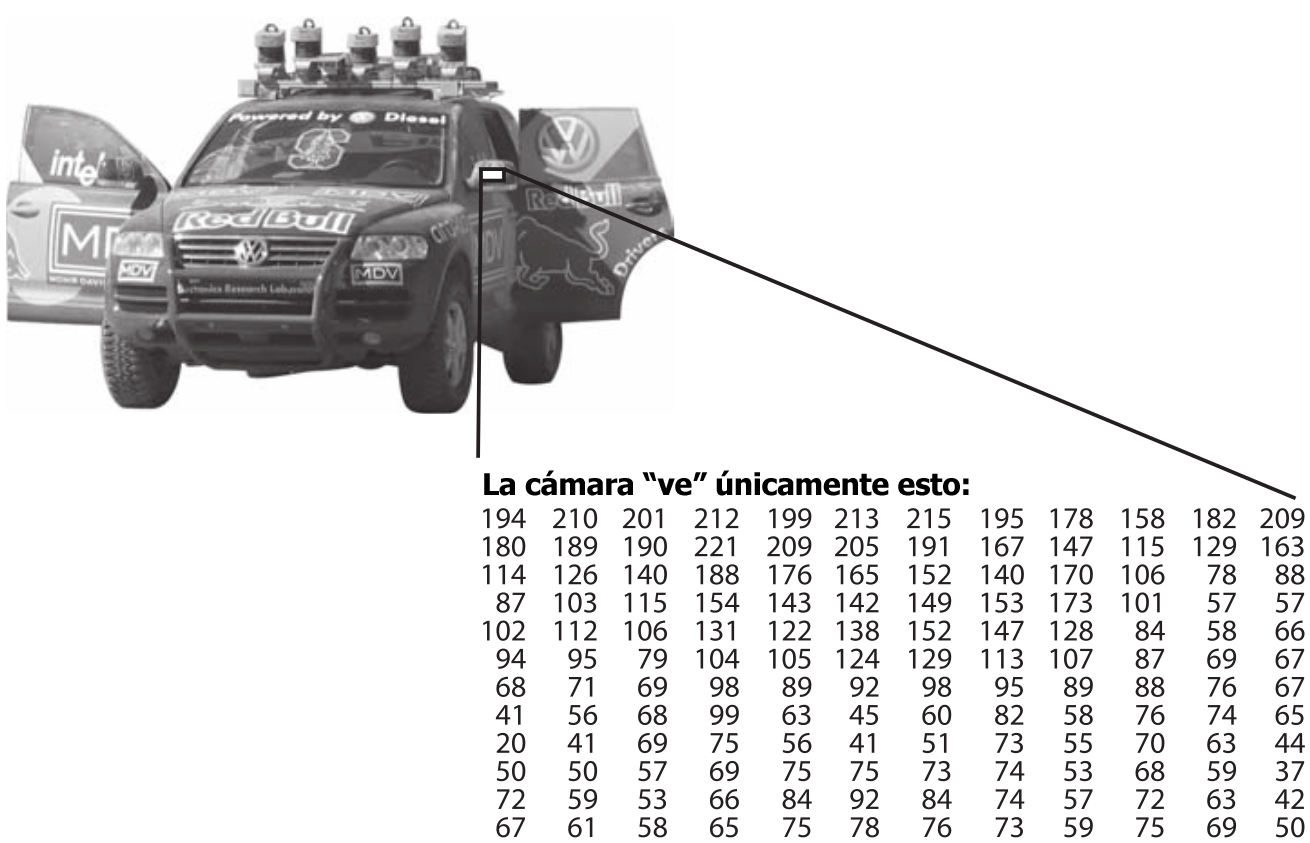
\includegraphics[width=1.0\textwidth]{images/fig1.png}
\caption[Lo que las computadoras ven en \emph{Visi\'{o}n Artificial}]%
{Para una computadora, el espejo retrovisor del carro es simplemente una matriz de n\'{u}meros. Imagen tomada del libro \emph{Learning OpenCV} \copyright \cite{Bradski_Kaehler_2008}.}
\label{fig:WhatComputersSee}
\end{figure}

Utilizando \'{u}nicamente la informaci\'{o}n brindada por una o m\'{a}s im\'{a}genes, se debe aplicar una serie de t\'{e}cnicas para determinar e interpretar su contenido y en el caso de procesos tridimensionales, recuperar la dimensi\'{o}n perdida (profundidad). La figura ~\ref{fig:WhatComputersSee} muestra la imagen de un autom\'{o}vil. En esa figura el ser humano es capaz de identificar f\'{a}cilmente el retrovisor del lado del conductor. Lo que una computadora \emph{ve} es simplemente una matriz de n\'{u}meros. Cada uno de los n\'{u}meros de esa matriz posee un amplio rango de \emph{ruido} y por lo tanto brinda muy poca informaci\'{o}n, pero esa matriz es todo lo que la computadora \emph{ve}.

\begin{figure}[H]
\centering
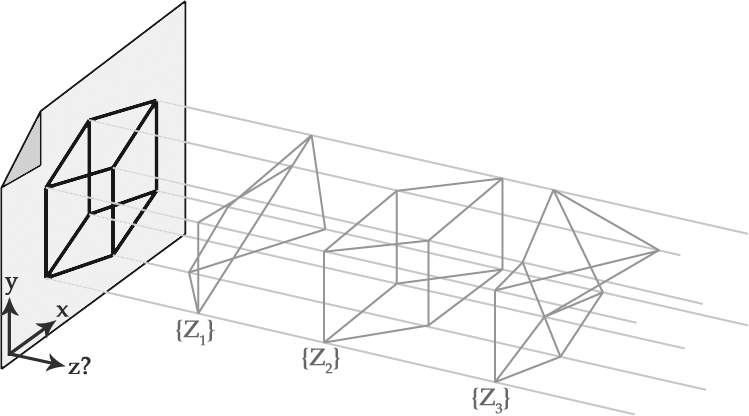
\includegraphics[width=1.0\textwidth]{images/2dto3dambiguity.png}
\caption[Problema de ambiguedad de una vista bidimensional (2D) de un mundo tridimensional (3D)]%
{Dada una vista bidimensional (2D) de un mundo tridimensional (3D), no existe una \'{u}nica o definitiva forma de reconstruir la señal 3D.}
\label{fig:2Dto3Dambiguity}
\end{figure}

Dada una vista bidimensional (2D) de un mundo tridimensional (3D), no existe una forma \'{u}nica o definitiva de reconstruir la señal 3D. De hecho el problema, es formalmente imposible de resolver \cite{Faugeras_Luong_2001,Bradski_Kaehler_2008,Hartley_Zisserman_2003}. La misma imagen 2D puede representar una colecci\'{o}n infinita de escenas 3D, a\'{u}n cuando los datos sean perfectos. En la figura ~\ref{fig:2Dto3Dambiguity} se muestra el problema de ambigüedad al reconstruir un cubo tridimensional a partir de una imagen bidimensional.

Los datos 2D se encuentran corruptos por ruido y distorsiones \cite{Freeman_Szeliski_2006,Thong_Sim_Phang_2001} provenientes del mundo real (clima, luz, reflecci\'{o}n, movimientos, sombras), de imperfecciones en el lente y construcci\'{o}n mec\'{a}nica de la c\'{a}mara, del ruido el\'{e}ctrico en el sensor u otros dispositivos electr\'{o}nicos y de la compresi\'{o}n de la imagen despu\'{e}s de ser capturada \cite{Szeliski_2010,Shah_1983,Faugeras_Luong_2001}.

A pesar de estas limitaciones, es posible utilizar conocimiento contextual adicional al diseñar un sistema pr\'{a}ctico, con tal de lidiar con los problemas impuestos por sensores visuales.

\section{Reconstrucci\'{o}n tridimensional}

\begin{figure}[H]
\centering
\subfloat[Reconstrucci\'{o}n pasiva de un objeto]{\label{fig:Pasive3DReconstruction}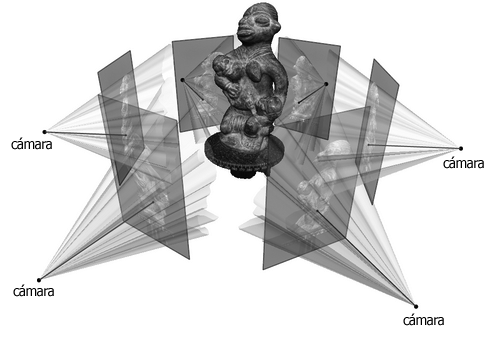
\includegraphics[width=0.5\textwidth]{images/pasive.png}}                
\subfloat[Reconstrucci\'{o}n activa de un objeto]{\label{fig:Active3DReconstruction}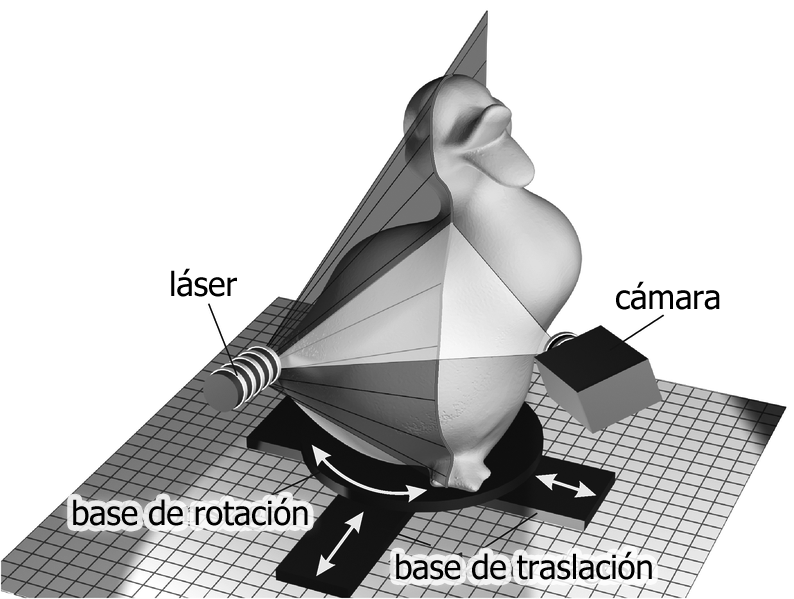
\includegraphics[width=0.5\textwidth]{images/active.png}}
\caption[Reconstrucci\'{o}n pasiva vs activa de un objeto tridimensional]%
{(a). Captura de im\'{a}genes durante el proceso pasivo de reconstrucci\'{o}n del objeto tridimensional. Imagen tomada de \url{http://carlos-hernandez.org/research.html} \copyright. (b). Proyecci\'{o}n de luz l\'{a}ser durante el proceso activo de re\-cons\-truc\-ci\'{o}n del objeto tridimensional. Imagen tomada de \url{http://en.wikipedia.org/wiki/File:LaserPrinciple.png} \copyright.}
\label{fig:3DReconstruction}
\end{figure}

La reconstrucci\'{o}n tridimensional es el proceso de capturar digitalmente la forma y apariencia de un objeto real. Este proceso puede ser realizado utilizando \emph{t\'{e}cnicas activas} o \emph{pasivas} \cite{Szeliski_2010,Forsyth_Ponce_2002,Cyganek_Siebert_2009}.

Al utilizar una \emph{t\'{e}cnica activa} de reconstrucci\'{o}n se interfiere activamente con el objeto. Generalmente, utiliza la proyecci\'{o}n de alg\'{u}n tipo de energ\'{i}a (luz l\'{a}ser o in\-fra\-rro\-ja) para lograr la reconstrucci\'{o}n. El c\'{a}lculo de la distancia tridimensional hacia los puntos del objeto se realiza por medio de la energ\'{i}a reflejada. Ejemplos de este tipo de t\'{e}cnica son c\'{a}maras in\-fra\-rro\-jas de profundidad, l\'{a}ser \emph{time-of-flight}, microondas o ultrasonido \cite{Rocchini_Cignoni_Montani_Pingi_Scopigno_2001,wiki:Janus_machine,Smisek_Jancosek_Pajdla_2011}. 

Por otro lado, al utilizar una \emph{t\'{e}cnica pasiva} de reconstrucci\'{o}n no se interfiere con el objeto. Generalmente, se utiliza un sensor con el cual se mide la radiaci\'{o}n reflejada o emitida por su superficie para determinar su estructura tridimensional. El sensor puede ser una c\'{a}mara fotogr\'{a}fica o de video sensible a la luz natural y los datos necesarios para la reconstrucci\'{o}n son el grupo de im\'{a}genes digitales (una o m\'{a}s) capturadas por \'{e}sta. El resultado final es una reconstrucci\'{o}n basada en im\'{a}genes \cite{Cyganek_Siebert_2009, Jahne_Haussecker_Geibler_1999, Faugeras_1992, Pollefeys_Gool_2002}. En la figura ~\ref{fig:3DReconstruction} se muestran las etapas de captura de im\'{a}genes (t\'{e}cnica pasiva) y proyecci\'{o}n de luz l\'{a}ser (t\'{e}cnica activa) para la reconstrucci\'{o}n de un objeto tridimensional.

Usualmente, un sistema completo de reconstrucci\'{o}n tridimensional se divide en tres grandes \'{a}reas: \emph{calibraci\'{o}n}, \emph{estimaci\'{o}n de la profundidad} y \emph{reconstrucci\'{o}n}.

\subsection{Calibraci\'{o}n}
Para determinar la profundidad a partir de una secuencia de im\'{a}genes es necesario realizar una calibraci\'{o}n de los puntos visuales de la c\'{a}mara y determinar sus par\'{a}metros extr\'{i}nsecos e intr\'{i}nsecos \cite{Jahne_Haussecker_Geibler_1999, Forsyth_Ponce_2002,Cyganek_Siebert_2009,Tsai_R_Y_1987}. En la figura ~\ref{fig:Calibration} se muestra una de las t\'{e}cnicas m\'{a}s populares de calibraci\'{o}n en la visi\'{o}n artificial utilizando un tablero de ajedrez.

\begin{figure}[H]
\centering
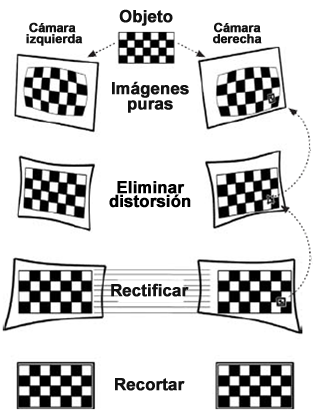
\includegraphics[width=0.4\textwidth]{images/calibration2.png}
\caption[T\'{e}cnica de calibraci\'{o}n utilizando un tablero de ajedrez]%
{La t\'{e}cnica de calibraci\'{o}n con tablero de ajedrez es una de las m\'{a}s po\-pu\-la\-res en la visi\'{o}n artificial. El proceso es necesario para revertir distorsiones en las im\'{a}genes causadas por la naturaleza mec\'{a}nica y electr\'{o}nica de las c\'{a}maras digitales. Imagen tomada de \url{http://meiyou.org/test2011/GSoC/} \copyright.}
\label{fig:Calibration}
\end{figure}

El proceso de calibraci\'{o}n permite determinar los par\'{a}metros necesarios para posteriormente corregir distorsiones en las im\'{a}genes generadas por el sistema de c\'{a}maras \cite{Bradski_Kaehler_2008,Shah_1983,Szeliski_2010, Tsai_R_Y_1987}. En la reconstrucci\'{o}n tridimensional se puede utilizar un aparejo con un par de c\'{a}maras (visi\'{o}n est\'{e}reo) calibradas \textit{a priori}. El problema de esta t\'{e}cnica est\'{a} en la dificultad de construir el aparejo y posicionar ambas c\'{a}maras con amplia precisi\'{o}n para obtener resultados aceptables en las im\'{a}genes estereosc\'{o}picas, limitando as\'{i} el uso pr\'{a}ctico del sistema \cite{Faugeras_Toscani_1986, Faugeras_Luong_2001, Faugeras_1993}. Por otro lado, es posible utilizar una secuencia de im\'{a}genes monosc\'{o}picas no calibradas generadas por una \'{u}nica c\'{a}mara y realizar la calibraci\'{o}n a partir de estos datos (auto-calibraci\'{o}n) \cite{Maybank_Faugeras_1992,Hartley_1993,Werner_Zisserman_2002,Hartley_Zisserman_2003}.

\subsection{Estimaci\'{o}n de la profundidad}
Es la etapa m\'{a}s compleja y desafiante del todo el proceso de reconstrucci\'{o}n tridimensional dado que hay que calcular la dimensi\'{o}n perdida (profundidad) a partir de im\'{a}genes bidimensionales. La estimaci\'{o}n de la profundidad se realiza utilizando \'{u}nicamente la informaci\'{o}n contenida en pares de im\'{a}genes es\-te\-reos\-c\'{o}pi\-cas, obtenidas por ejemplo por el sensor \emph{\ac{CCD}} de una c\'{a}mara.

Para estimar un modelo tridimensional de la escena se debe encontrar pareos entre pixeles de las im\'{a}genes y convertir sus posiciones 2D en posiciones 3D \cite{Cyganek_Siebert_2009, Szeliski_2010,Shah_1983}. A la distancia entre un pixel en una imagen y el mismo pixel en la otra imagen se le conoce como \emph{disparidad} \cite{Cyganek_Siebert_2009,Forsyth_Ponce_2002,Shah_1983}. Tal distancia es inversamente proporcional a la distancia de la profundidad y puede ser calculada por triangulaci\'{o}n.

Al resultado final de este proceso se le conoce como nube de puntos tridimensionales (del ingl\'{e}s \textit{point cloud}). En la figura ~\ref{fig:PointCloud} se muestra una nube de puntos calculados a partir de una secuencia de im\'{a}genes no calibradas.

\begin{figure}[H]
\centering
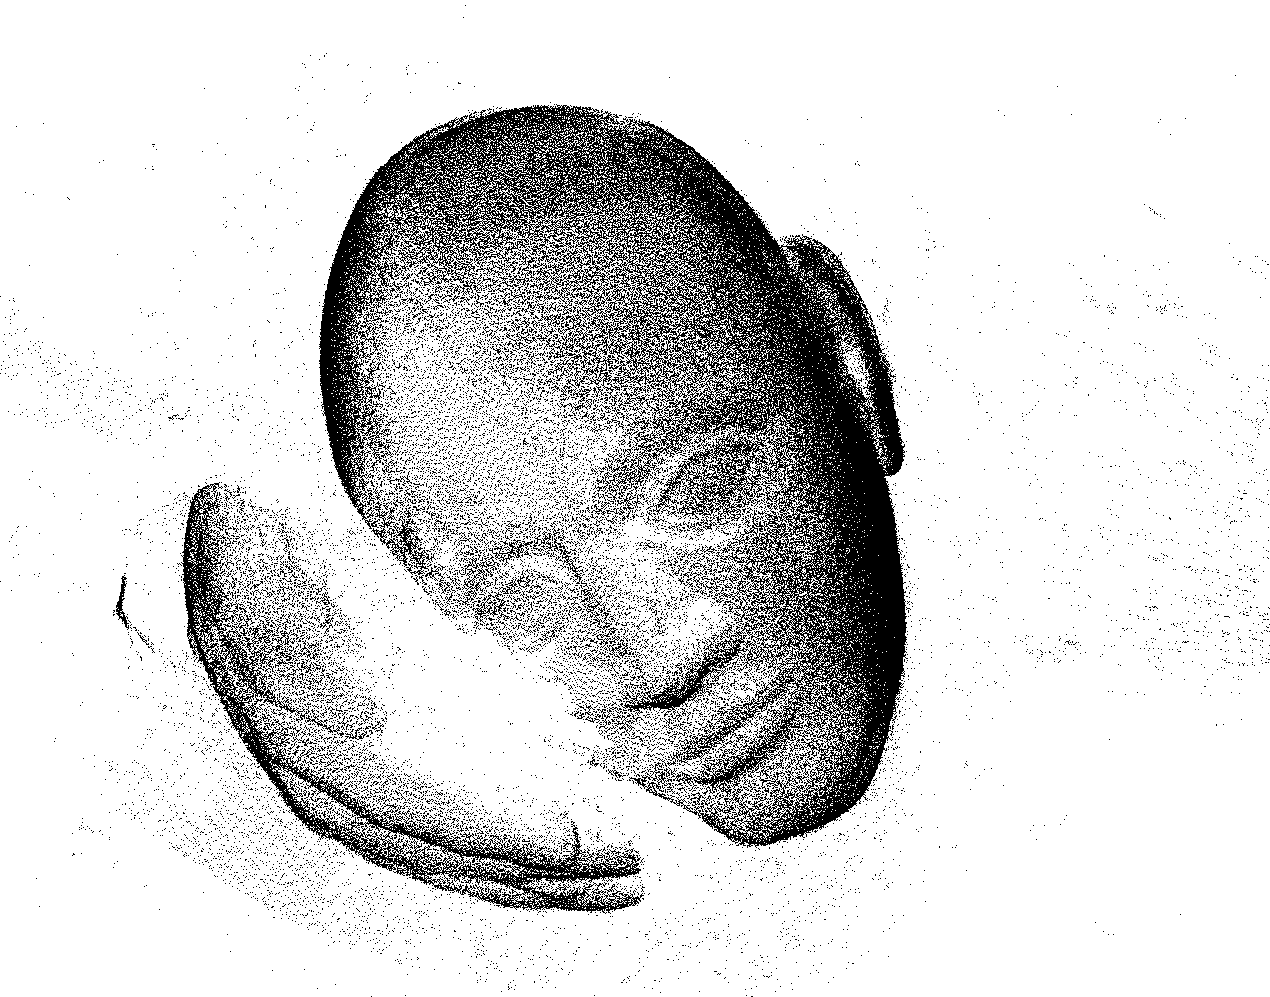
\includegraphics[width=0.6\textwidth]{images/point_cloud_b.png}
\caption[Nube de puntos calculada a partir de un objeto tridimensional]%
{Nube de puntos calculada a partir de una secuencia de im\'{a}genes no calibradas. Imagen tomada de \url{http://cmp.felk.cvut.cz/projects/is3d/} \copyright.}
\label{fig:PointCloud}
\end{figure}

\subsection{Reconstrucci\'{o}n}
La reconstrucci\'{o}n completa del objeto empieza con las diferentes nubes de puntos obtenidas en la fase anterior. Para modelar de forma completa (360\degree) un objeto se evaluan diferentes vistas para mejorar la geometr\'{i}a en reconstrucci\'{o}n (proceso conocido como \textbf{refinamiento}) \cite{Jahne_Haussecker_Geibler_1999,Cyganek_Siebert_2009}. Los grupos de puntos obtenidos se registran en un sistema de coordenadas consistente para obtener mapas de profundidad robustos (proceso conocido como \textbf{registro}). Finalmente, se convierten los diferentes mapas en una serie de modelos tridimensionales y se fusiona en un \'{u}nico modelo \cite{Cyganek_Siebert_2009, Bardsley_2008, Jahne_Haussecker_Geibler_1999, pan2009ProFORMA}. En la figura ~\ref{fig:3DModel} se muestra el resultado final de la reconstrucci\'{o}n completa del objeto.

\begin{figure}[H]
\centering
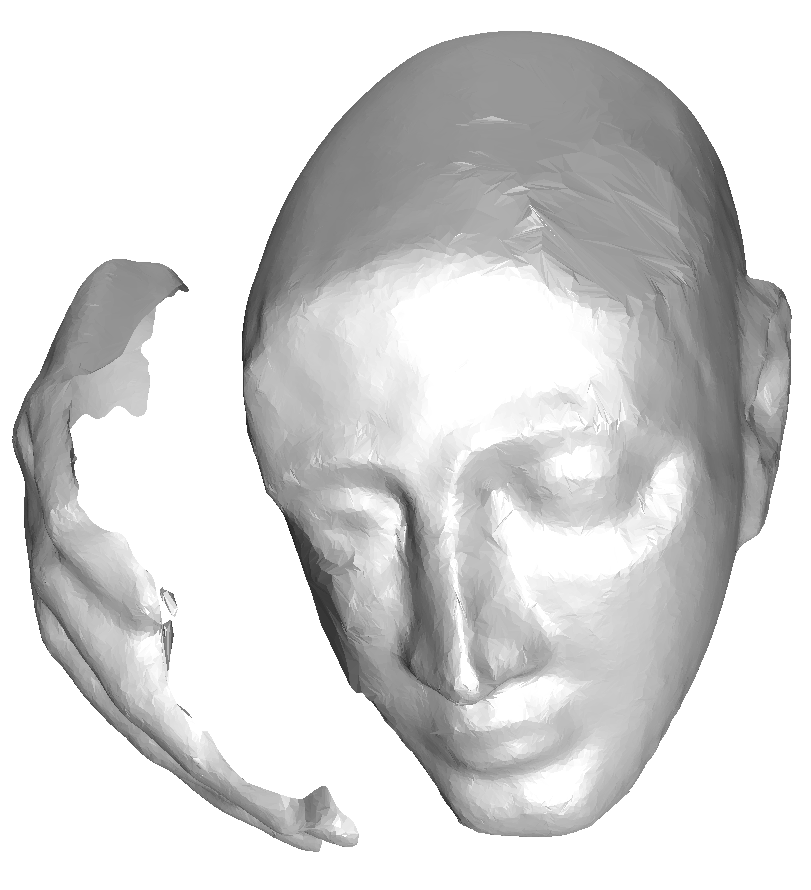
\includegraphics[width=0.45\textwidth]{images/Head-crust-faired-snap3.png}
\caption[Modelo de superficie tridimensional]%
{Modelo de superficie tridimensional obtenido a partir del proceso de refinamiento y fusi\'{o}n de los mapas de profundidad obtenidos a partir de las nubes de puntos. Imagen tomada de \url{http://cmp.felk.cvut.cz/projects/is3d/} \copyright.}
\label{fig:3DModel}
\end{figure}


\section{Trabajo relacionado}
Pan Q. et al. \cite{pan2009ProFORMA} proponen una t\'{e}cnica de reconstrucci\'{o}n basada en la utilizaci\'{o}n de descriptores para determinar la apariencia tridimensional del objeto. El problema de su t\'{e}cnica es que limita la reconstrucci\'{o}n a objetos con geometr\'{i}as muy simples (como cilindros y cubos), genera una cantidad excesiva de pol\'{i}gonos incluso en objetos simples y su reconstrucci\'{o}n es totalmente dispersa (pocos puntos). La t\'{e}cnica propuesta en este documento va m\'{a}s all\'{a} que reconstruir cilindros o cubos y pretende realizar una reconstrucci\'{o}n densa aprovechando todas las caracter\'{i}sticas f\'{i}sicas del objeto (forma, textura, color).

Kyle McDonald et al. \cite{wiki:Janus_machine} presentan un sistema activo que utiliza proyectores digitales, esc\'{a}neres y la t\'{e}cnica de luz estructurada para reconstruir tridimensionalmente la cabeza de la persona que se coloque frente al esc\'{a}ner. La utilizaci\'{o}n de equipo caro especializado como los proyectores y esc\'{a}neres es indeseable as\'{i} como el tiempo que tarda la construcci\'{o}n del modelo 3D.

Faugeras et al. \cite{Faugeras_1992} describen el tipo de informaci\'{o}n tridimensional que puede obtenerse al utilizar un aparejo binocular est\'{e}reo sin calibraci\'{o}n. Su t\'{e}cnica no toma en cuenta el tiempo de reconstrucci\'{o}n y se enfoca m\'{a}s en su resultado final.

Hassner et al. \cite{Hassner_Basri_2006} describen una t\'{e}cnica de reconstrucci\'{o}n utilizando una sola imagen bidimensional m\'{a}s una base de datos de objetos tridimensionales. La utilizaci\'{o}n de cualquier tipo de informaci\'{o}n \textit{a priori} para guiar la reconstrucci\'{o}n va en contra de lo propuesto en esta tesis.

Rocchini et al. \cite{Rocchini_Cignoni_Montani_Pingi_Scopigno_2001} proponen la creación de un esc\'{a}ner tridimensional de bajo costo basado en luz estructurada. La utilizaci\'{o}n de t\'{e}cnicas activas de reconstrucci\'{o}n, como es el caso de luz estructurada, necesita equipo especializado y costoso.


\section{Organizaci\'{o}n del documento}
El cap\'{i}tulo \ref{chap:descripcion} brinda una descripci\'{o}n general de la investigaci\'{o}n realizada. Se detalla la hip\'{o}tesis de la tesis en conjunto con el experimento utilizado para comprobar su validez. Luego se enumeran los objetivos de la tesis y finalmente, se brinda una secci\'{o}n de aportes, alcances y limitaciones de la t\'{e}cnica de reconstrucci\'{o}n r\'{a}pida propuesta.

En el cap\'{i}tulo \ref{chap:calibracion} se detalla todo el proceso de calibraci\'{o}n del experimento. Este cap\'{i}tulo es la base para lograr una buena reconstrucci\'{o}n tridimensional.

En el cap\'{i}tulo \ref{chap:profundidad} se describe el proceso de estimaci\'{o}n de la profundidad de los puntos tridimensionales del objeto a reconstruir el cual se basa en el algoritmo de triangulaci\'{o}n iterativo de m\'{i}nimos cuadrados.

En el cap\'{i}tulo \ref{chap:reconstruccion} se describe c\'{o}mo utilizar las matrices de la c\'{a}mara en conjunto con el algoritmo de triangulaci\'{o}n para reconstruir tridimensionalmente el objeto. Primero se brinda una descripci\'{o}n de c\'{o}mo realizar el proceso utilizando un par de vistas estereosc\'{o}picas y posteriormente, se muestra c\'{o}mo extenderlo a m\'{a}s de dos vistas.

En el cap\'{i}tulo \ref{chap:algoritmo} se describe el pseudoc\'{o}digo del algoritmo de reconstrucci\'{o}n propuesto en esta tesis y posteriormente, las principales diferencias con t\'{e}cnicas similares de reconstrucci\'{o}n.

%En el cap\'{i}tulo \ref{chap:algoritmo} se describe el pseudoc\'{o}digo del algoritmo de reconstrucci\'{o}n propuesto en esta tesis. Adicionalmente, se brinda su an\'{a}lisis de complejidad y finalmente, las principales diferencias con t\'{e}cnicas similares de reconstrucci\'{o}n.

En el cap\'{i}tulo \ref{chap:resultados} se muestran los resultados obtenidos durante las diferentes pruebas a las que fue sometida la t\'{e}cnica propuesta utilizando dos tipos distintos de c\'{a}maras.

En el cap\'{i}tulo \ref{chap:analisis} se detalla el an\'{a}lisis de los datos obtenidos durante la ejecuci\'{o}n de las diferentes pruebas del experimento.

Finalmente, en el cap\'{i}tulo \ref{chap:conclusiones} se presentan las conclusiones de la investigaci\'{o}n y el trabajo realizado. Luego, se detalla una secci\'{o}n relacionada con posibles mejoras y trabajo futuro.

%@TODO mejorar la descripcion de cada capitulo
%@TODO necesita conclusion del chapter???
